% Chapter Template

\chapter{Ensayos y resultados} % Main chapter title

\label{Chapter4} % Change X to a consecutive number; for referencing this chapter elsewhere, use \ref{ChapterX}

Este capítulo presenta los ensayos realizados para evaluar el desempeño del prototipo y los resultados obtenidos. Los ensayos se desarrollaron para validar la funcionalidad y exactitud del sistema en condiciones operativas de laboratorio. Los objetivos principales de los ensayos fueron:


\begin{enumerate}

\item Validar la funcionalidad del hardware. Asegurar que todos los componentes del sistema funcionan correctamente y se comunican entre sí de manera eficiente.

\item Probar la integración del firmware. Verificar que el firmware gestiona adecuadamente la adquisición de datos, el procesamiento y la transmisión al \textit{broker} MQTT.

\item Evaluar la exactitud de la geolocalización GNSS. Medir la precisión de las coordenadas proporcionadas por el módulo GNSS y compararlas con un patrón de referencia.

\item Comprobar la visualización de la aplicación de mapas. Asegurar que la aplicación proporciona una representación útil de los datos GNSS recibidos.

\end{enumerate}

%----------------------------------------------------------------------------------------
%	SECTION 1
%----------------------------------------------------------------------------------------

\section{Resultado final de la integración del hardware}
\label{sec:proto_v_final}

En esta sección se presentan los resultados finales de la construcción del hardware. En la figura \ref{fig:proto_exterior} se muestra una vista externa de la versión final del prototipo construido. En la figura \ref{fig:proto_interior} se revela una vista interna del prototipo, donde se puede ver el cableado y los módulos de hardware conectadas a la placa base del sistema.

\begin{figure}[H]
	\centering
	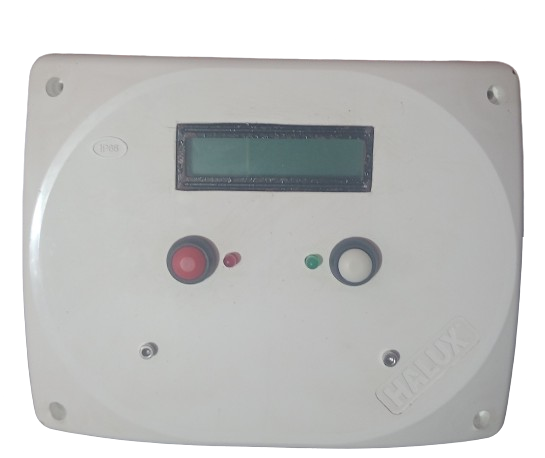
\includegraphics[width=.5\textwidth]{./Figures/Prototipo_v_final_exterior.png}
	\caption{Resultado final del hardware desarrollado (exterior).}
	\label{fig:proto_exterior}
\end{figure}

\begin{figure}[H]
	\centering
	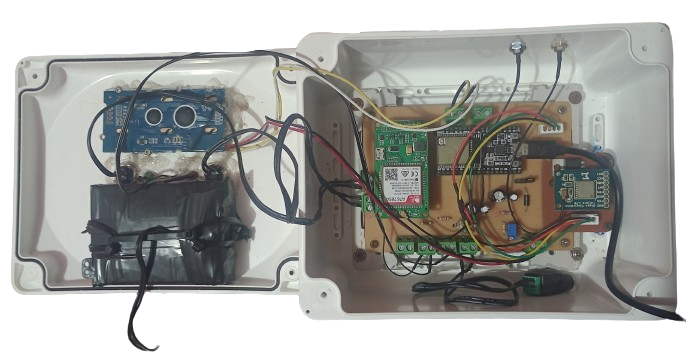
\includegraphics[width=.8\textwidth]{./Figures/Prototipo_v_final_interior.png}
	\caption{Resultado final del hardware desarrollado (interior).}
	\label{fig:proto_interior}
\end{figure}


En la figura \ref{fig:proto_componentes_ext} se señalan los siguientes componentes:

\begin{enumerate}
\item Pantalla LCD.
\item Botones y pilotos.
\end{enumerate}


\begin{figure}[H]
	\centering
	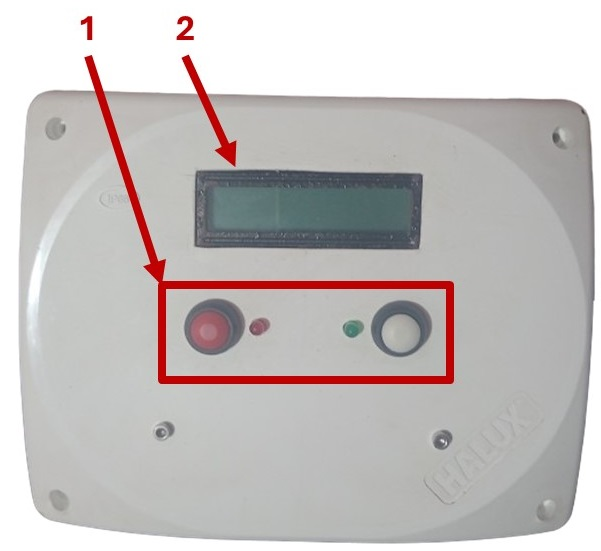
\includegraphics[width=.5\textwidth]{./Figures/Prototipo_v_final_exterior_componentes.jpg}
	\caption{Vista real de los componentes del hardware (exterior).}
	\label{fig:proto_componentes_ext}
\end{figure}


En la figura \ref{fig:proto_componentes_int} se señalan los siguientes componentes:

\begin{enumerate}
\item Batería.
\item Módulo SIM A7670SA.
\item ESP32.
\item Conectores SMA hembra para antena celular (izq.) y para antena GNSS (dcha.).
\item Módulo Quectel L76.
\end{enumerate}


\begin{figure}[H]
	\centering
	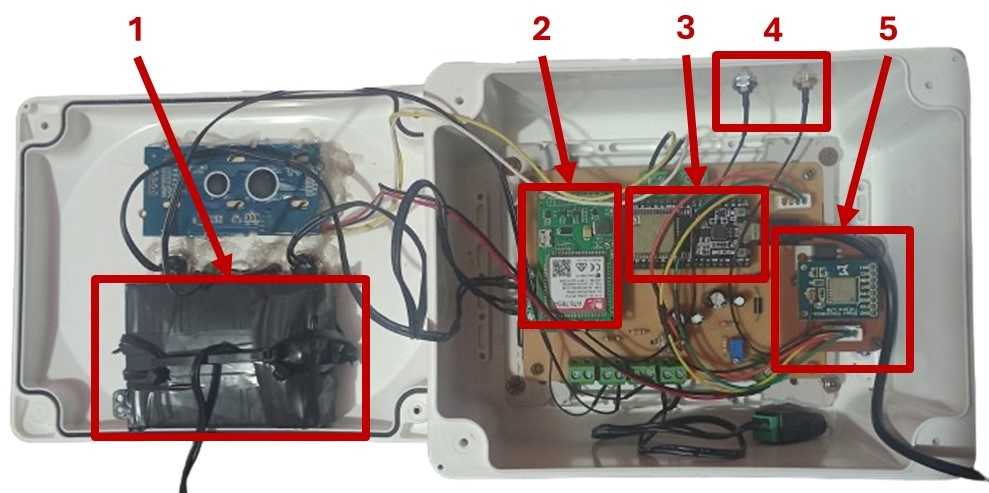
\includegraphics[width=.8\textwidth]{./Figures/Prototipo_v_final_interior_componentes.jpg}
	\caption{Vista real de los componentes del hardware (interior).}
	\label{fig:proto_componentes_int}
\end{figure}


%----------------------------------------------------------------------------------------
%	SECTION 2
%----------------------------------------------------------------------------------------


\section{Pruebas funcionales del hardware}
\label{sec:pruebasHW}

En esta sección se describe la metodología seguida para realizar las pruebas del hardware, se presentan los resultados que se obtuvieron y su correspondiente análisis.


\subsection{Metodología para las pruebas del hardware}

Se ejecutaron pruebas sobre los módulos de hardware para verificar que funcionan e interactúan adecuadamente entre sí. A continuación, se describe la metodología ejecutada: 

\begin{enumerate}
\item En la PCB desarrollada:
	\begin{enumerate}
	\item Se verificaron las conexiones de los componentes para observar que no existen contactos abiertos, en cortocircuito o fallas a tierra.
	\item Se verificó que a la salida del circuito de regulación se da un nivel de tensión de 5 VDC, necesarios para la alimentación de cada módulo.
	\item Se midió el consumo de corriente de todo el hardware a plena carga, es decir, realizando todas las tareas para las que fue diseñado. 
	\end{enumerate}

\item Se realizaron pruebas unitarias de comunicación entre los diferentes módulos montados sobre la PCB. Para esto, se realizó lo siguiente: 

	\begin{enumerate}
	
	\item  Se probó la recepción de tramas NMEA con el módulo Quectel L76, a través del puerto UART. Se construyó un código de prueba que capturó las tramas NMEA recibidas por puerto UART\_1 y su eco en el puerto UART\_0 para visualizar los datos recibidos en la computadora, a través de la terminal \textit{Hercules} \citep{hercules}. 
	
	\item Se probó la comunicación bidireccional con el módulo SIM A7670SA, a través del puerto UART y por comandos AT. Se construyó un código de prueba que captura las tramas AT, recibidas por puerto UART\_1 y su eco en el puerto UART\_0 para visualizar los datos recibidos en la computadora, a través de la terminal \textit{Hercules}; este mismo programa transmite las tramas AT enviadas desde el puerto UART\_0 hasta el módulo SIM A7670SA en el UART\_1. De esta manera, se pueden enviar comandos AT de forma manual hacia el módulo y recibir las respuestas respectivas. 
	
	\item Se realizó un código de prueba para utilizar todas las funciones proporcionadas por el driver \verb|lcd_i2c_grove.h| y verificar la visualización correcta de textos predefinidos en la pantalla. 
	
	\end{enumerate}
	
\end{enumerate}


\subsection{Resultados y análisis}

\subsubsection{De las pruebas sobre la PCB}

Se verificó que no existen contactos abiertos, cortocircuitos o fallas a tierra antes y después del proceso de soldadura de la PCB. Se verificó la salida del circuito de regulación, y se observa una salida de 4.9 VDC suficiente para la alimentación de los módulos que componen el sistema, en la figura \ref{fig:prueba_regulador} se muestra una fotografía de la prueba. 

\begin{figure}[H]
	\centering
	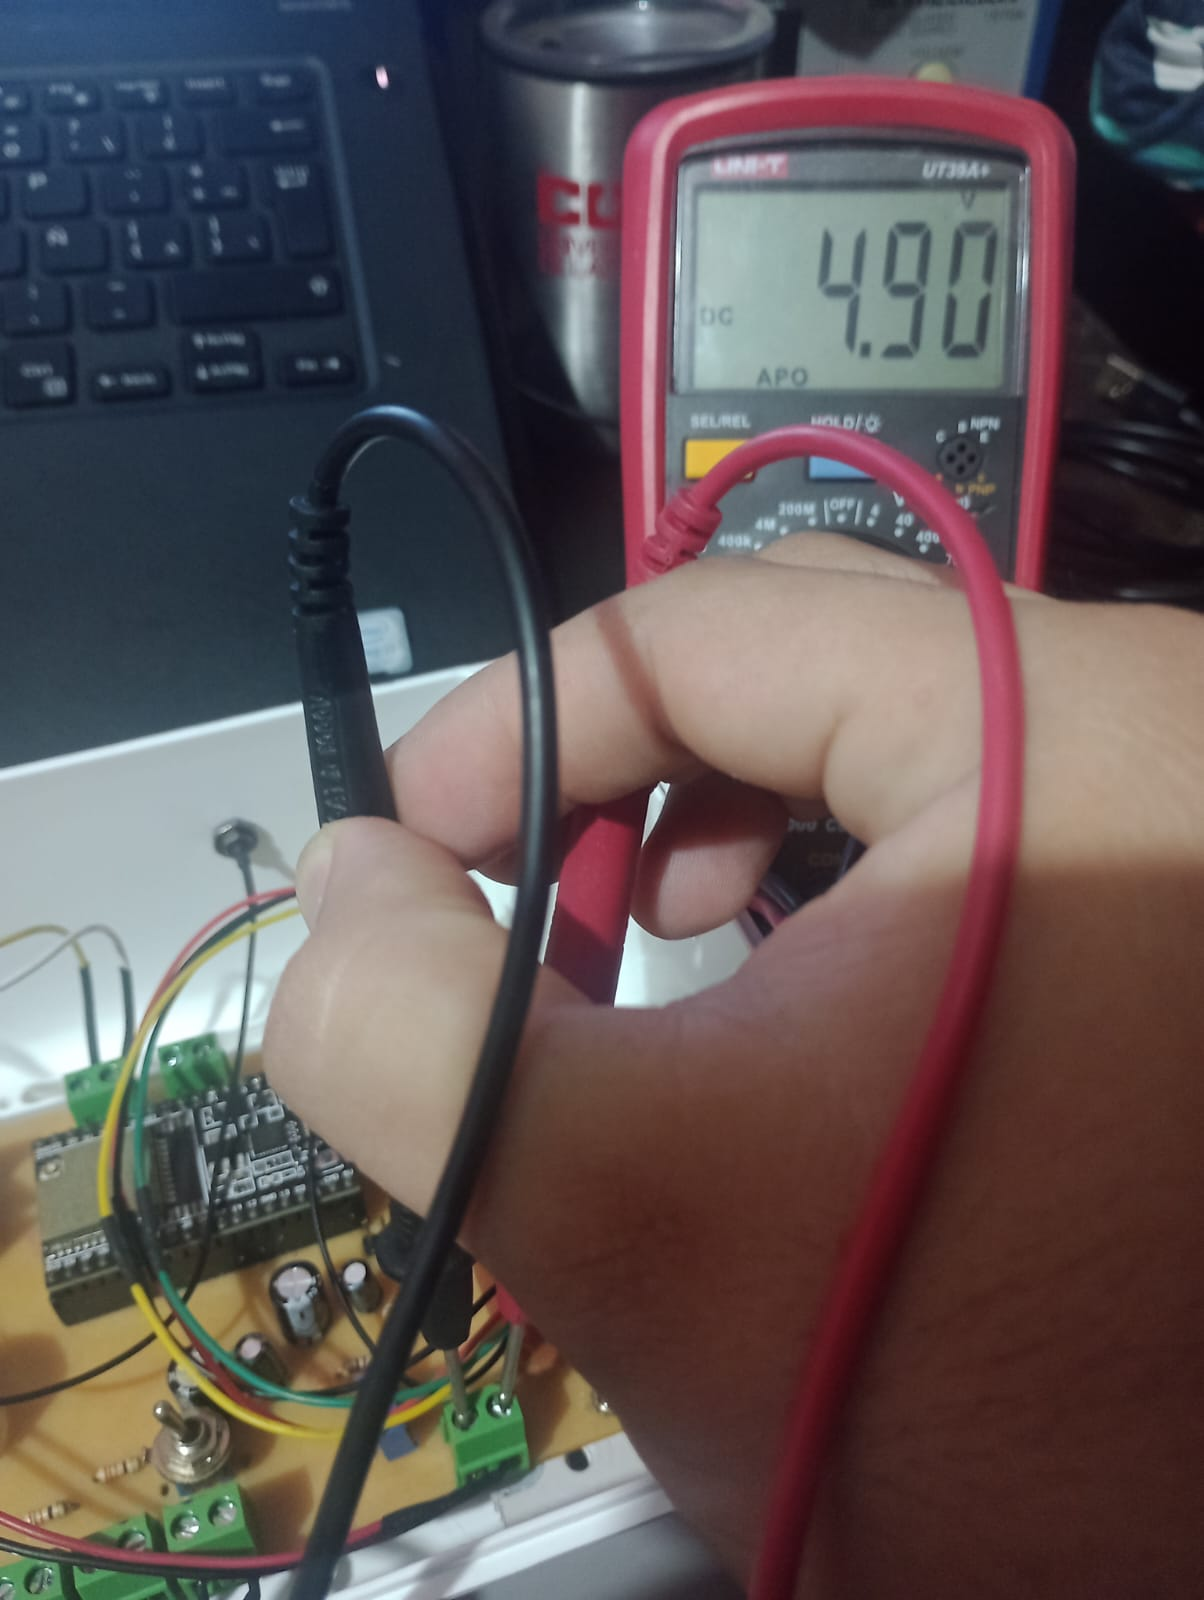
\includegraphics[width=.5\textwidth]{./Figures/Prueba_regulador.jpeg}
	\caption{Medición de la salida en el circuito de regulación.}
	\label{fig:prueba_regulador}
\end{figure}

La medición de la corriente total consumida por el hardware se llevó a cabo por un período de 30 segundos contado a partir de que se enciende el dispositivo; este es el tiempo que le toma al sistema inicializarse y comenzar a enviar datos al servidor.  Resultó que existen variaciones desde los 130 mA hasta los 190 mA. La medición mostró valores con picos de 210 mA. 

Se observó que los mayores picos de corriente se dan cuando el módulo SIM A7670SA recién se conecta a la red celular. También, se observa que el valor de corriente que más se repite en las mediciones es 150 mA. En la figura \ref{fig:graf_corr} se muestra el gráfico de las muestras tomadas; la secuencia de valores corresponde temporalmente, es decir, que describe el comportamiento de la corriente en el tiempo. Además, en la figura \ref{fig:pru_corr_datos_repre} se muestran fotografías de las mediciones más representativas. 

\begin{figure}[H]
	\centering
	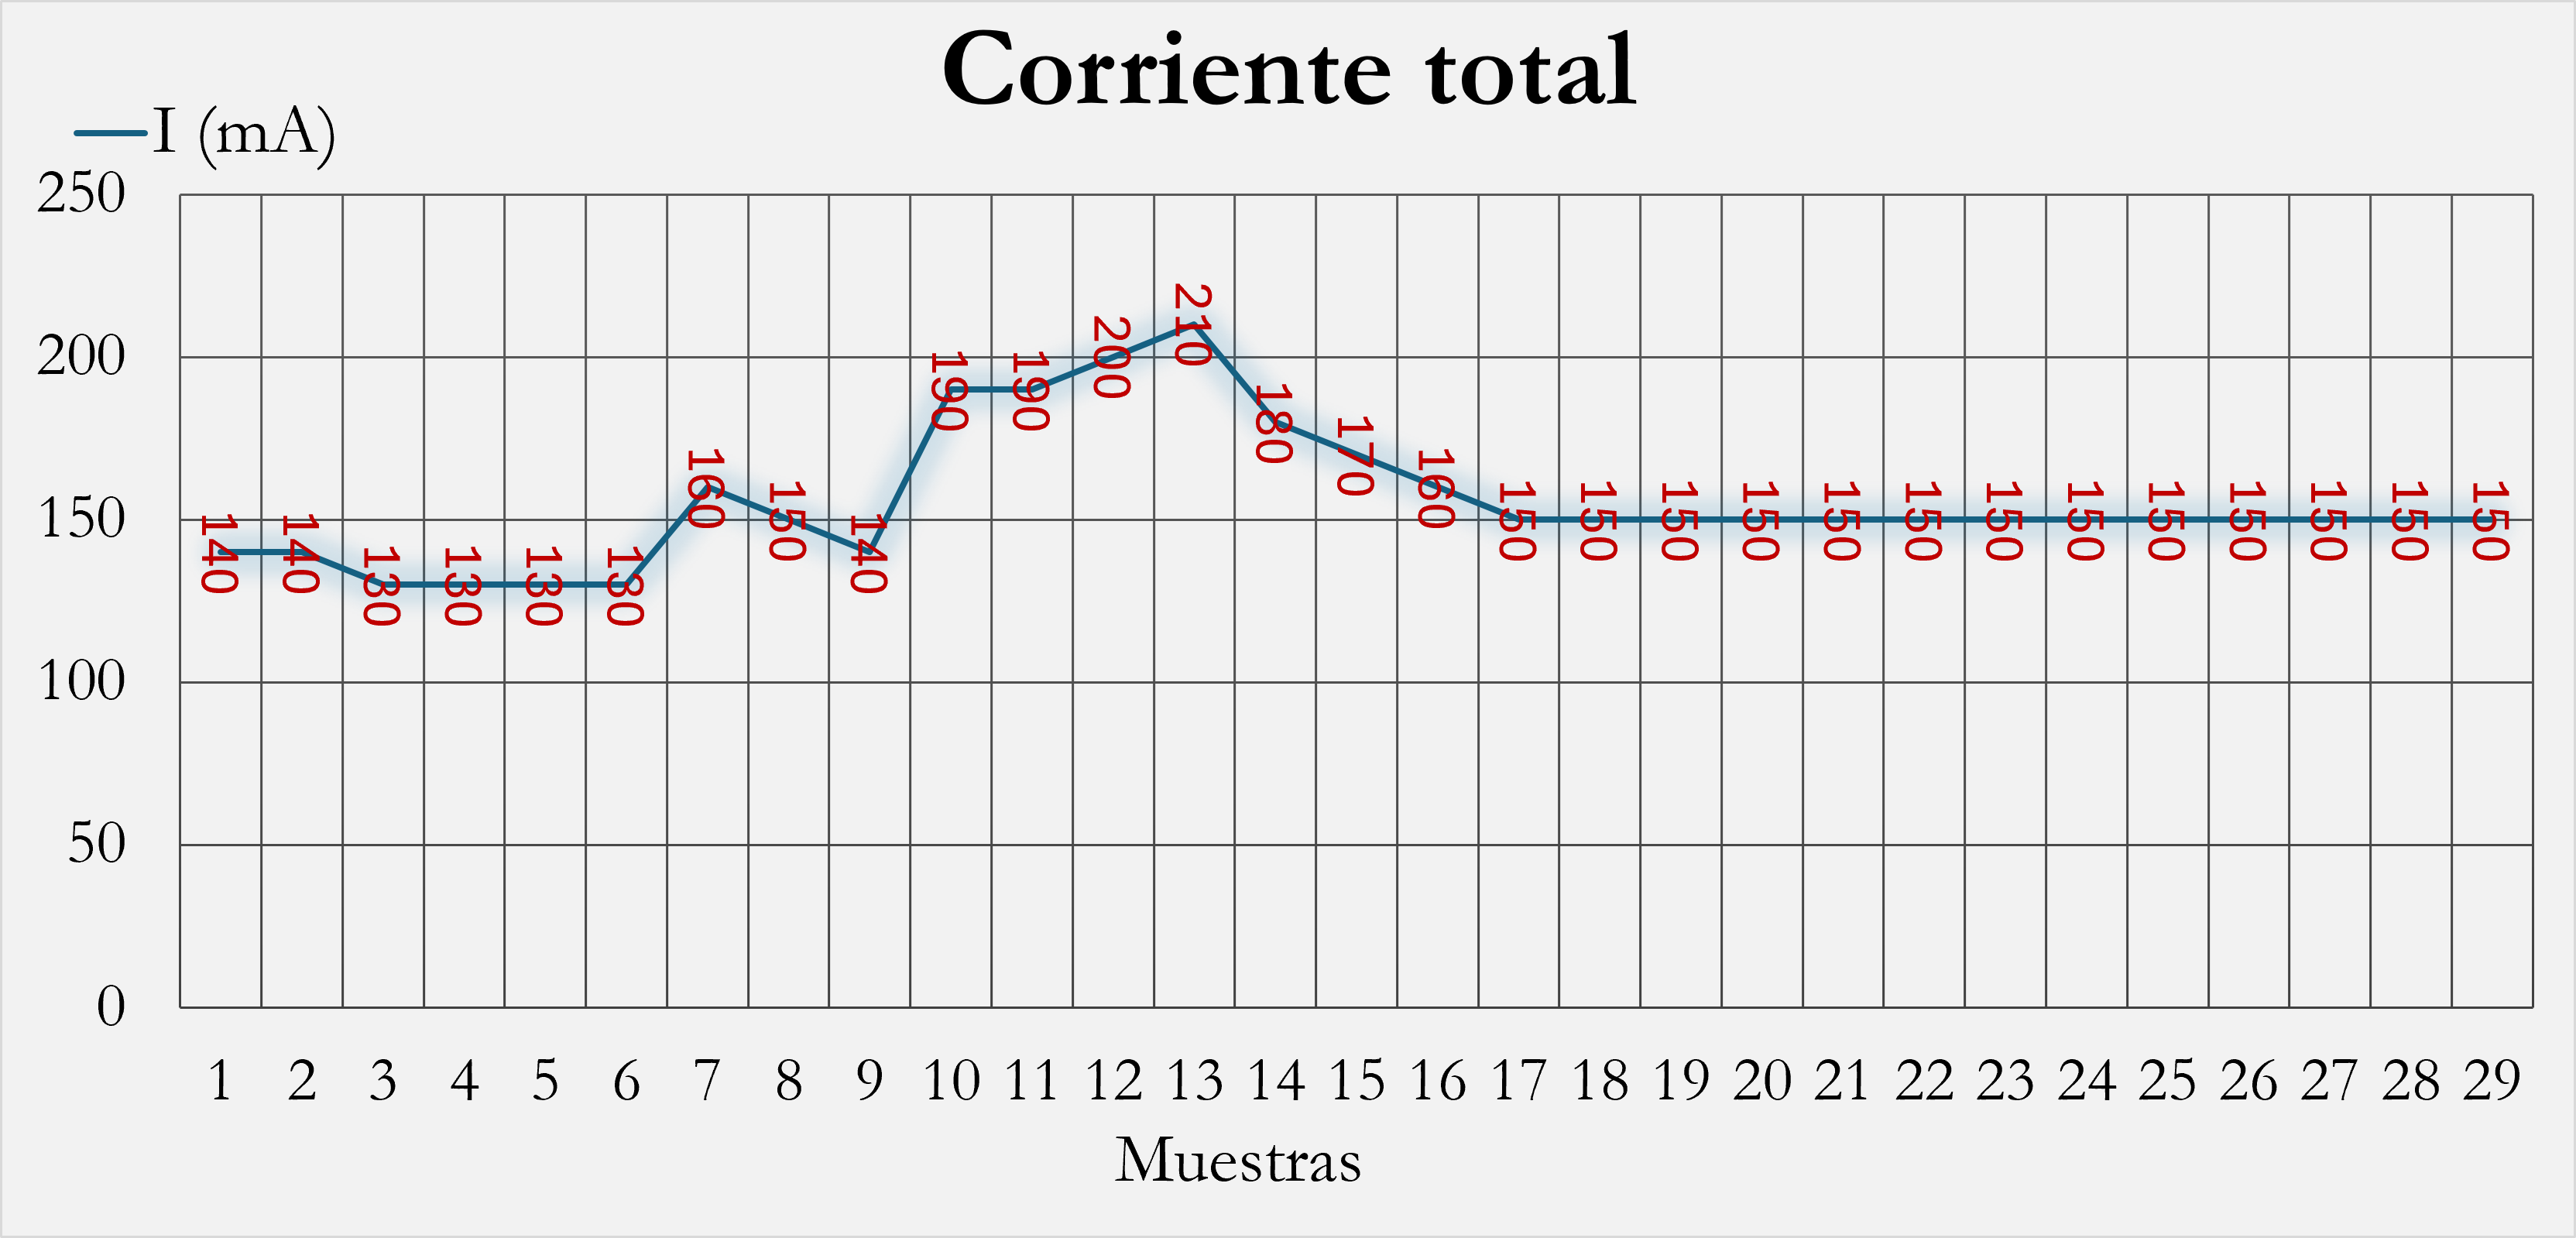
\includegraphics[width=1\textwidth]{./Figures/grafico_corriente.png}
	\caption{Gráfico de la muestras tomadas en la medición de corriente.}
	\label{fig:graf_corr}
\end{figure}

\begin{figure}[H]
	\centering
	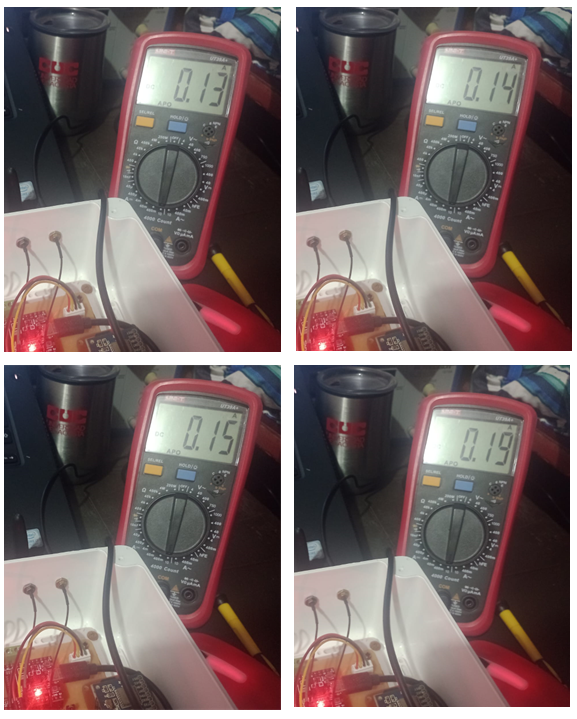
\includegraphics[width=.6\textwidth]{./Figures/Prueba_corriente_datos_repre.png}
	\caption{Datos más representativos en la medición de corriente.}
	\label{fig:pru_corr_datos_repre}
\end{figure}


\subsubsection{De las pruebas entre módulos}

\textbf{Prueba del módulo Quectel L76} 

En la figura \ref{fig:pru_QL76_Diag} se muestra un diagrama de la conexión necesaria para esta prueba. En la figura \ref{fig:pru_QL76_Setup} se muestra la conexión real realizada. En esta configuración se realiza lo siguiente: 

\begin{enumerate}
\item Se intercambias los pines GND, Vin, Tx y Rx del módulo Quectel L76 en la ranura del módulo SIM A7670SA. Debido a que son conectores diferentes se deben emplear cables de prueba. Lo anterior, para poder usar el puerto UART\_1.

\item Se deben desconectar los módulos SIM A7670SA y Quectel L76 de sus respectivas posiciones designadas, para interferir la comunicación serial. 
\end{enumerate}

\begin{figure}[H]
	\centering
	
\includegraphics[width=.7\textwidth]{./Figures/prueba_QL76_diagrama.png}
	\caption{Diagrama de conexiones para la prueba del módulo Quectel L76.}
	\label{fig:pru_QL76_Diag}
\end{figure}

\begin{figure}[H]
	\centering
	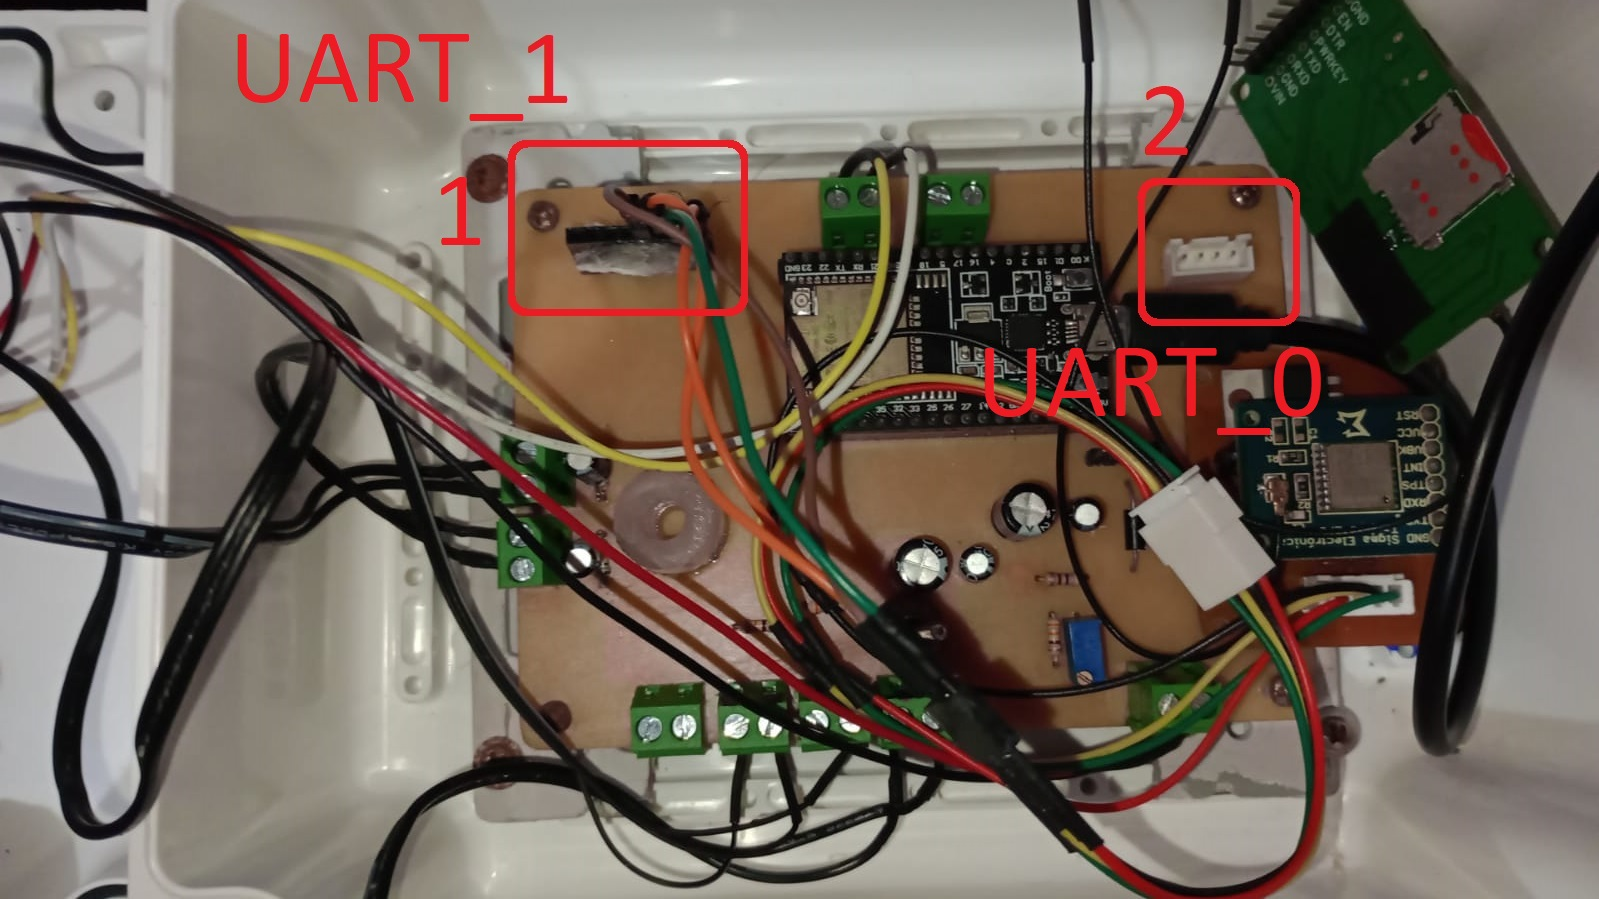
\includegraphics[width=.8\textwidth]{./Figures/prueba_QL76_Setup.jpeg}
	\caption{Conexiones reales para la prueba del módulo Quectel L76.}
	\label{fig:pru_QL76_Setup}
\end{figure}


El código de prueba implementado es el que se muestra en el código \ref{cod:cod_proof_gnss}. Por simplicidad y reducir el espacio en este documento, se han obviado las declaraciones de variables, macros y la función \verb|main()|. Este sencillo programa utiliza \textit{FreeRTOS} para crear dos tareas, la primera \verb|uart1_interrupt_task()|, que se encarga de recibir las tramas del puerto UART\_1 (donde está conectado el módulo L76) y retransmitirlas al computador por el puerto UART\_0; y la segunda \verb|uart0_interrupt_task()| permite enviar comandos PMTK desde le computador hacia el módulo L76. De esta manera se comprueba que hay una comunicación adecuada entre los módulos. La función \verb|main()| se encarga de incializar los puertos UART en modo de interrupciones y crear las tareas correspondientes. 

\begin{figure}[H]
\begin{lstlisting} 
static void uart1_interrupt_task(void *params)
{
    uart_event_t uart_event;
    uint8_t *uart_recv_data = (uint8_t *)malloc(BUF_SIZE);
    while (1)
    {
        if (xQueueReceive(uart1_queue, &uart_event, portMAX_DELAY))
        {
            bzero(uart_recv_data, BUF_SIZE);
            switch (uart_event.type)
            {
            case UART_DATA:
                uart_receive(UART1, uart_recv_data, uart_event.size);
                uart_transmit(UART0, uart_recv_data, strlen(uart_recv_data));
                bzero(uart_recv_data, BUF_SIZE);
                break; 
            }
        }
    }
    free(uart_recv_data);
}
static void uart0_interrupt_task(void *params)
{
    uart_event_t uart_event;
    uint8_t *uart_recv_data = (uint8_t *)malloc(BUF_SIZE);
    while (1)
    {
        if (xQueueReceive(uart0_queue, &uart_event, portMAX_DELAY))
        {
            bzero(uart_recv_data, BUF_SIZE);

            switch (uart_event.type)
            {
            case UART_DATA:
                uart_receive(UART0, uart_recv_data, uart_event.size);
                uart_transmit(UART1, uart_recv_data, strlen(uart_recv_data));
                break; 
            }
        }
        
    }
    free(uart_recv_data);
}

\end{lstlisting}
\captionof{lstlisting}{Código para probar comunicación con el módulo Quectel L76.}
\label{cod:cod_proof_gnss}
\end{figure}


Luego de implementar las configuraciones anteriores, se obtuvieron las tramas NMEA proporcionadas por el módulo Quectel L76. La prueba resultó exitosa, ya que es posible capturar dichas tramas y procesarlas. En la figura \ref{fig:pru_QL76_recep} se muestra una captura de las tramas visualizadas en la terminal \textit{Hercules}. En esta captura se puede observar las tramas que incian con \$GNRMC, las cuales contienen la información de geolocalización del módulo.  

\begin{figure}[H]
	\centering
	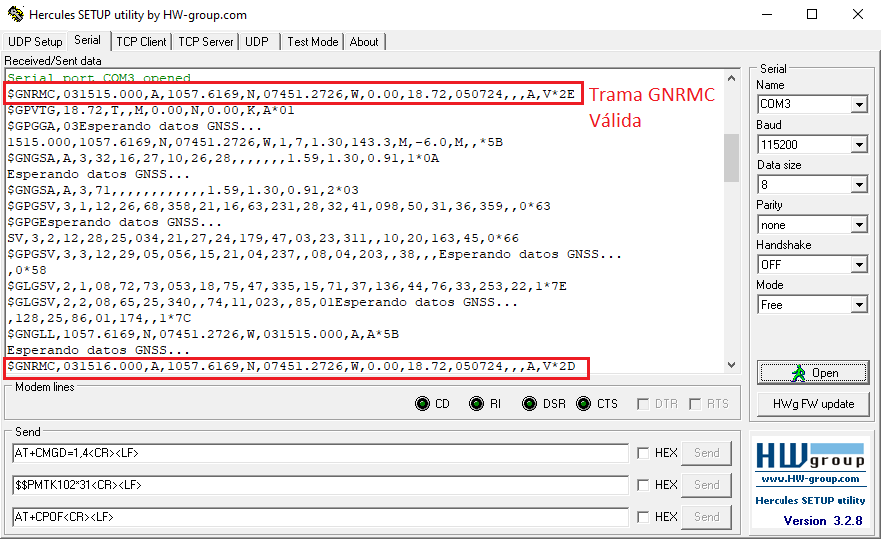
\includegraphics[width=1\textwidth]{./Figures/prueba_QL76_recepcion_ana.png}
	\caption{Vista de las tramas NMEA en la terminal \textit{Hercules}.}
	\label{fig:pru_QL76_recep}
\end{figure}



\textbf{Prueba del módulo SIM A7670SA}


En la figura \ref{fig:pru_A7670_Diag} se muestra un diagrama de la conexión necesaria para esta prueba. En la figura \ref{fig:pru_A7670_Setup} se muestra la conexión real realizada. En esta configuración se realiza lo siguiente: 

\begin{enumerate}
\item Se mantiene conectado el módulo SIM A7670SA ya que tiene designado el puerto UART\_1.

\item Se desconecta el módulo Quectel L76 de su ranura, para que no interfiera la comunicación serial por el puerto UART\_0.
\end{enumerate}

\begin{figure}[H]
	\centering
	
\includegraphics[width=.7\textwidth]{./Figures/prueba_A7670SA_diagrama.png}
	\caption{Diagrama de conexiones para la prueba del módulo Quectel L76.}
	\label{fig:pru_A7670_Diag}
\end{figure}

\begin{figure}[H]
	\centering
	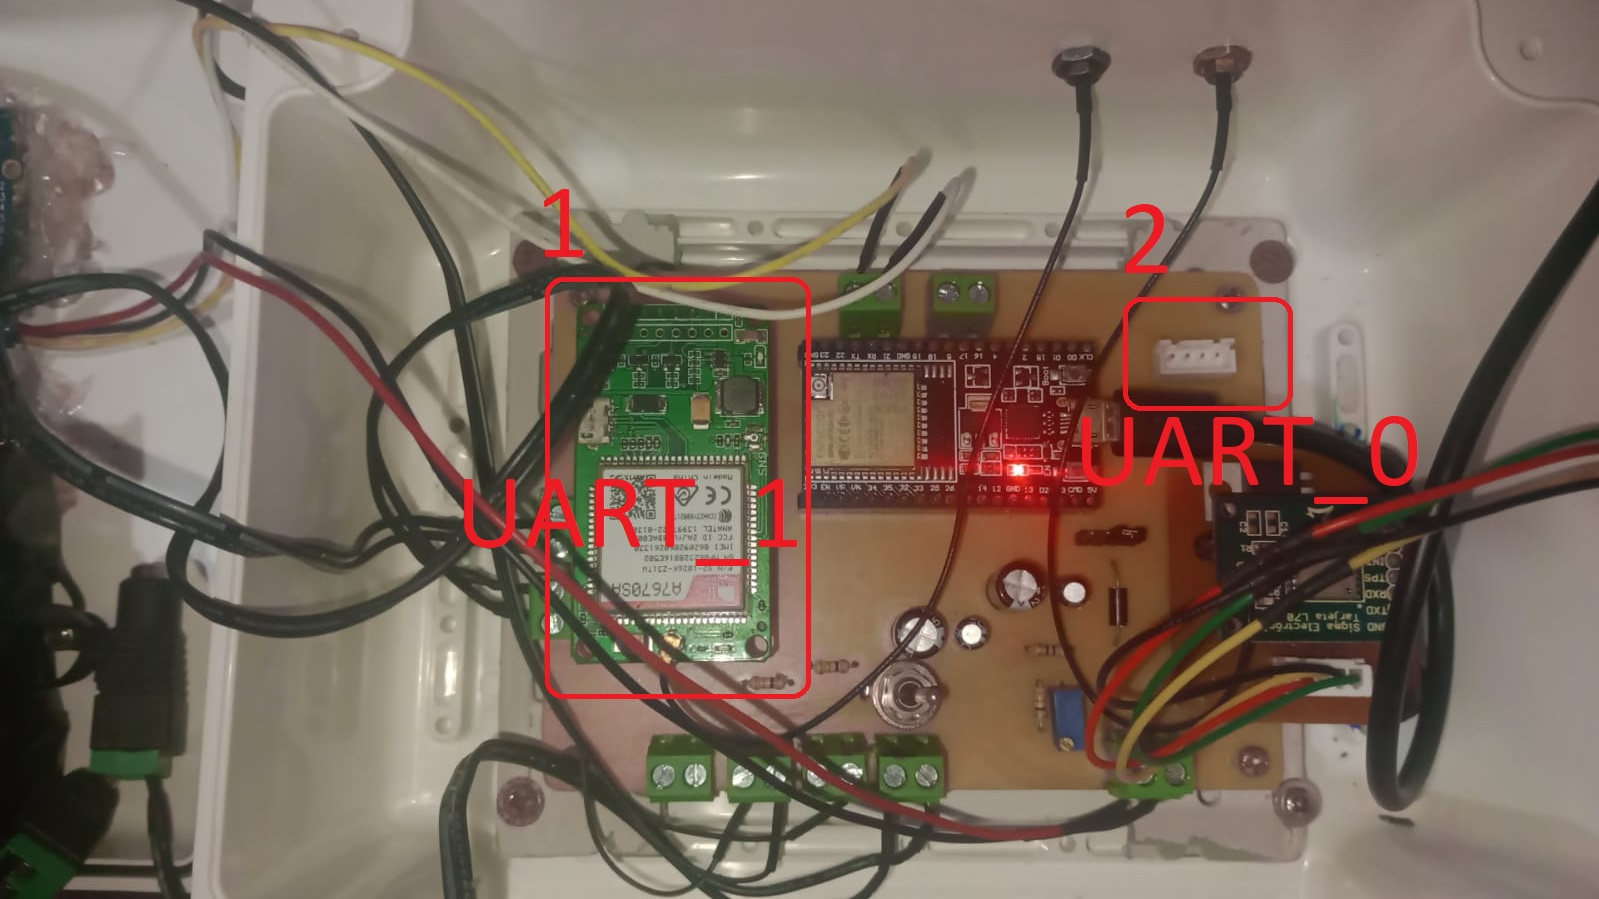
\includegraphics[width=.8\textwidth]{./Figures/Prueba_A7670SA_Setup.jpeg}
	\caption{Conexiones reales para la prueba del módulo Quectel L76.}
	\label{fig:pru_A7670_Setup}
\end{figure}


El código de prueba implementado es el mismo que se implementó en la prueba anterior (ver código \ref{cod:cod_proof_gnss}). Igual que en la prueba anterior, la tarea \verb|uart1_interrupt_task()|, se encarga de recibir las tramas del puerto UART\_1 (donde está conectado el módulo SIM A7670SA) y retransmitirlas al computador por el puerto UART\_0; y la tarea \verb|uart0_interrupt_task()| permite enviar comandos AT desde le computador hacia el módulo SIM A7670SA, de forma manual desde la terminal \textit{Hercules}. 

Luego de implementar las configuraciones anteriores, se obtuvieron las tramas AT que responde el módulo SIM A7670SA y se pudieron transmitir comandos AT hacia este módulo. La prueba resultó exitosa, ya que es posible capturar dichas tramas y procesarlas. 

En la figura \ref{fig:pru_A7670_recep} se muestra una captura de los mensajes visualizados en la terminal \textit{Hercules}. En esta captura se puede observar mensajes recibidos del módulo SIM A7670SA que inician los símbolos + y *, los cuales contienen información sobre los procesos del módulo.   

\begin{figure}[H]
	\centering
	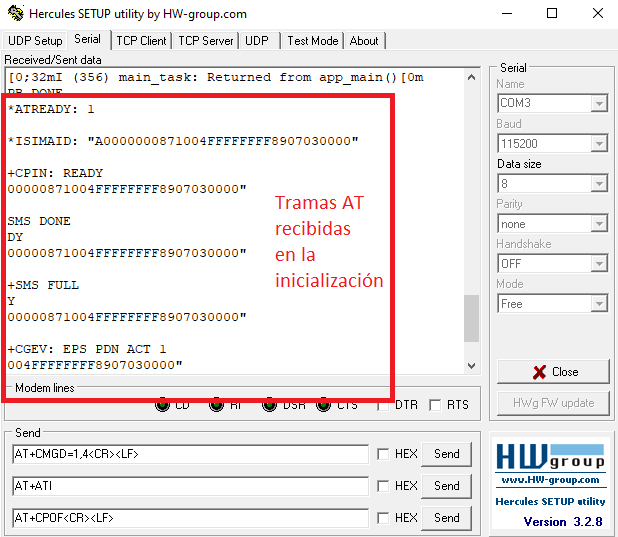
\includegraphics[width=1\textwidth]{./Figures/Prueba_A7670SA_recep_AT.png}
	\caption{Vista de las tramas AT en la terminal \textit{Hercules}.}
	\label{fig:pru_A7670_recep}
\end{figure}

En la figura \ref{fig:pru_A7670_transm} se muestra otra captura de mensajes visualizados en la terminal \textit{Hercules}. En esta captura se muestra la transmisión del comando \textbf{AT+CMGD=1,4} hacia el módulo SIM A7670SA, este comando de be cumplir con las siguientes condiciones: 

\begin{enumerate}
\item Debe iniciar con los caracteres \textbf{AT+}.
\item Seguido del comando a enviar. En el caso de la prueba realizada, se envió el comando CMGD que se usa para eliminar mensajes SMS. 
\item Los parámetros del comando. en este caso <index>(1), <delflag>(4), para borrar todos los mensajes en la tarjeta SIM.
\item Por último, los símbolos de retorno de carro <CR> y salto de línea <LF>. Si estos dos símbolos no están presentes, el comando no será reconocido.
\end{enumerate}

En la figura \ref{fig:pru_A7670_transm} también se observa en la figura la respuesta del módulo al comando recibido. El módulo responde con un texto que contiene el comando recibido y 'OK' para indicar que el comando fue ejecutado con éxito. 

\begin{figure}[H]
	\centering
	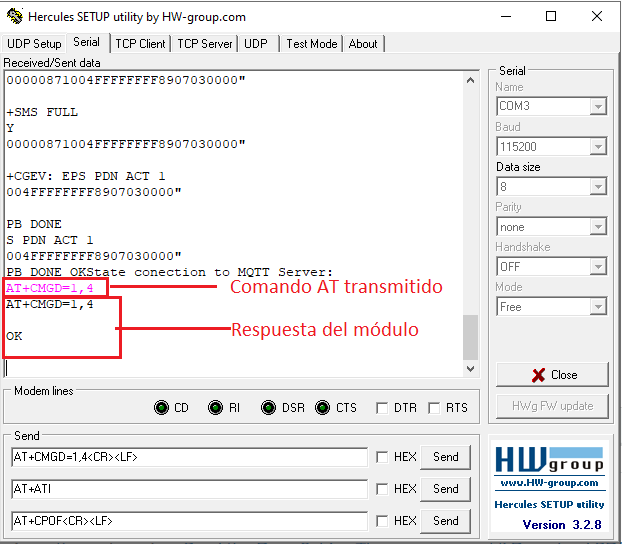
\includegraphics[width=1\textwidth]{./Figures/Prueba_A7670SA_transmision_AT.png}
	\caption{Vista de las tramas AT en la terminal \textit{Hercules}.}
	\label{fig:pru_A7670_transm}
\end{figure}



\textbf{Prueba de la pantalla LCD}


Para esta prueba no es necesaria ninguna configuración especial, más allá de las conexiones de diseño del hardware. 

Se implementó un código de prueba (ver código \ref{cod:cod_proof_lcd}) que permitió usar las funciones proporcionadas por el driver \verb|lcd_i2c_grove.h|. Este sencillo programa escribe textos y cambia los colores de la pantalla LCD cada 3 segundos, además que borra la pantalla cada vez que escribe un texto nuevo. De esta manera se puede corroborar el funcionamiento de la LCD. en la figura \ref{fig:prueba_lcd} se muestran fotografías de los resultados de la prueba. 

\begin{figure}[H]
\begin{lstlisting}
void app_main()
{
    lcd_init(); 
    lcd_clear(); lcd_set_RGB(255, 255, 255); //pantalla blanca
    lcd_write(0, 0, "Linea 0"); lcd_write(1, 0, "Linea 1");
    delay(DELAY_LCD);

    while(1)
    {
        lcd_clear(); 
        lcd_write(0, 0, "Color: "); lcd_write(1, 0, "Rojo");
        lcd_set_RGB(255, 0, 0); //pantalla roja
        delay(DELAY_LCD);

        lcd_clear(); 
        lcd_write(0, 0, "Color: "); lcd_write(1, 0, "Verde");
        lcd_set_RGB(0, 255, 0); //pantalla verde
        delay(DELAY_LCD);

        lcd_clear(); 
        lcd_write(0, 0, "Color: "); lcd_write(1, 0, "Azul");
        lcd_set_RGB(0, 0, 255); //pantalla azul
        delay(DELAY_LCD);

        lcd_clear(); 
        lcd_write(0, 0, "Color: "); lcd_write(1, 0, "amarillo");
        lcd_set_RGB(255, 255, 0); //pantalla amarilla
        delay(DELAY_LCD);

        lcd_clear(); 
        lcd_write(0, 0, "Color: "); lcd_write(1, 0, "magenta");
        lcd_set_RGB(255, 0, 255); //pantalla magenta
        delay(DELAY_LCD);

        lcd_clear(); 
        lcd_write(0, 0, "Color: "); lcd_write(1, 0, "Cyan");
        lcd_set_RGB(0, 255, 255); //pantalla cyan
        delay(DELAY_LCD);
    }
}

\end{lstlisting}
\captionof{lstlisting}{Código para probar comunicación con la pantalla LCD.}
\label{cod:cod_proof_lcd}
\end{figure}



\begin{figure}[H]
	\centering
	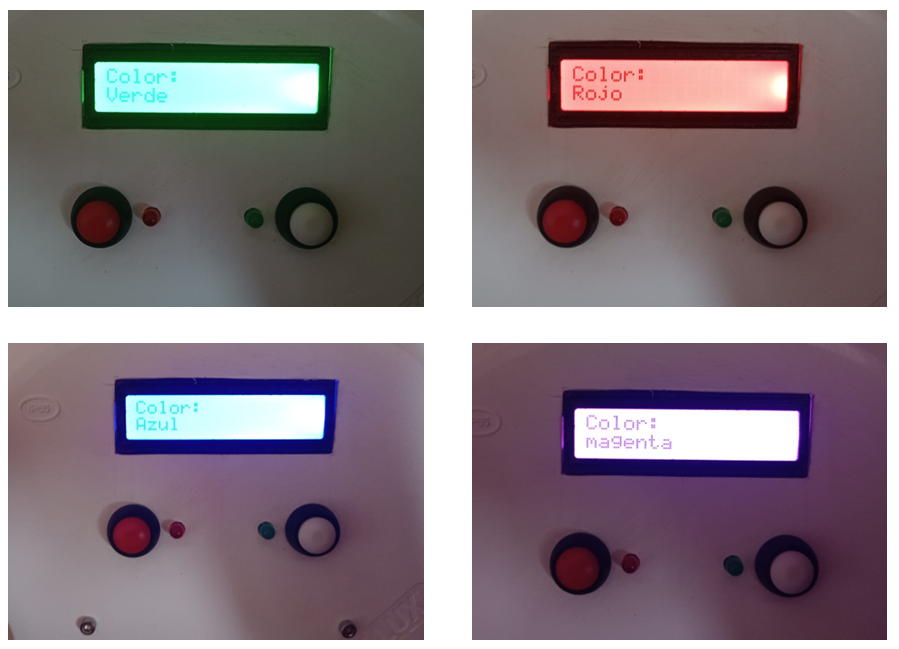
\includegraphics[width=1\textwidth]{./Figures/prueba_LCD_collage.png}
	\caption{Fotos de la prueba de la pantalla LCD.}
	\label{fig:prueba_lcd}
\end{figure}





%----------------------------------------------------------------------------------------
%	SECTION 3
%----------------------------------------------------------------------------------------



\section{Pruebas funcionales de la aplicación web}
\label{sec:pruebasWeb}

En esta sección se describe la metodología seguida para realizar las pruebas de la aplicación web, se presentan los resultados que se obtuvieron y su correspondiente análisis.

Las pruebas llevadas a cabo fueron las siguientes:

\begin{enumerate}
\item Prueba de integración con el hardware.
\item Prueba de exactitud de la ubicación.
\end{enumerate}


\subsection{Prueba de integración con el hardware}

En este escenario se probó la capacidad de la aplicación web para conectarse con el \textit{broker} EMQX y procesar la información que transmite el hardware. Para esto, se ejecutaron los siguientes pasos: 

\subsubsection{Metodología}

\begin{enumerate}
\item Se puso en funcionamiento normal el hardware. 
\item Se accedió al enlace donde se aloja la página web del servicio de mapas.
\item Se comprobó la recepción de la ubicación actual en una trayectoria de 100 m. 
\end{enumerate}

\subsubsection{Resultados y análisis}

En la figura \ref{fig:prueba_web_1_mapa} se muestra la aplicación de web con el mapa y la trayectoria descrita por el movimiento del hardware. En esta prueba el recorrido se hizo a pie debido a la corta distancia a recorrer. Se obtuvo una respuesta adecuada de la interacción del sistema completo, desde la recepción de la geolocalización, la transmisión de la información al \textit{broker} a través de internet en la red celular, hasta la visualización en la web. 

\begin{figure}[H]
	\centering
	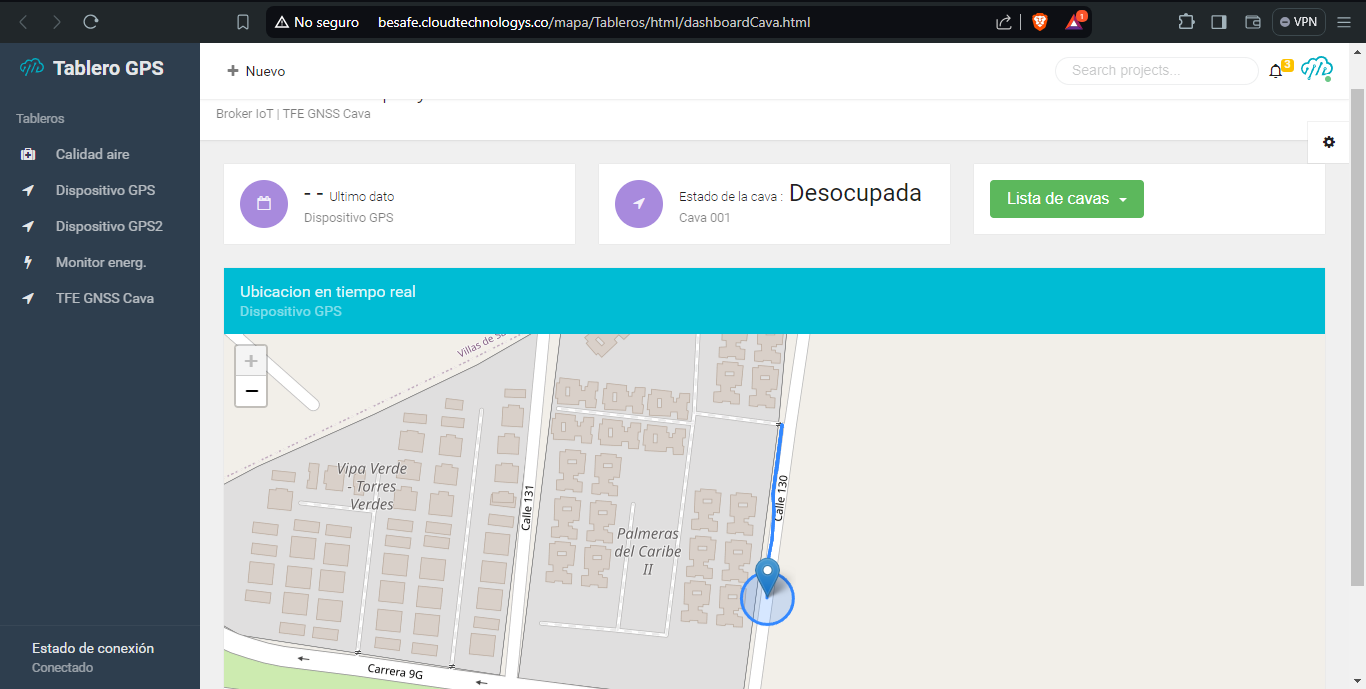
\includegraphics[width=1\textwidth]{./Figures/prueba_web_1_mapa.png}
	\caption{Captura del mapa para la prueba de integración con el hardware.}
	\label{fig:prueba_web_1_mapa}
\end{figure}


\subsection{Prueba de exactitud de la ubicación}

Para realizar esta prueba, se procedió a verificar la exactitud de la localización que proporciona el hardware. Para esto, se capturaron los datos de posición en diversos escenarios y se compararon las coordenadas obtenidas con las coordenadas reales conocidas. A continuación, se describe la metodología llevada a cabo:

\subsubsection{Metodología}

\begin{enumerate}
\item Se seleccionaron posiciones en puntos fijos en la ciudad de Barranquilla. En un conjunto de edificios residenciales con calles internas para recrear espacios urbanos con presencia de edificios y también cuenta con zonas abiertas. 

\item Se marcaron las coordenadas geográficas de los puntos seleccionados. para esto se utilizó la aplicación \textit{Google Map} y un teléfono inteligente como instrumento patrón. 

\item En cada punto de prueba se registraron las coordenadas proporcionadas por el prototipo y por el teléfono inteligente. Se tomaron cinco muestras con una separación de un minuto. El valor de la medición que se seleccionó fue el que más se repite de las cinco muestras. 

\item Se calculó la distancia entre las coordenadas registradas por el prototipo y las coordenadas tomadas de referencia de \textit{Google Map}. El cálculo de esta distancia se realizó con la ecuación de \textit{Haversine}. El cálculo se toma como el grado de exactitud en la geolocalización realizada por el prototipo.

\end{enumerate}


\subsubsection{Resultados y análisis}

Luego de realizadas las pruebas se obtuvieron se tabularon los datos obtenidos (ver tabla \ref{tabla:distancias_calculadas}). 


\begin{table}[h]
    \centering
    \caption{Mediciones de la exactitud en la geolocalización}
    \begin{tabular}{p{.7cm} p{2cm} p{2.2cm} p{2cm} p{2.3cm} p{2.2cm}}
    \toprule
        & \multicolumn{2}{p{4.2cm}}{\textbf{Prototipo}} & \multicolumn{2}{p{4.3cm}}{\textbf{Google Maps}} &    \\
        \textbf{\#} & \textbf{Latitud 1} & \textbf{Longitud 1} & \textbf{Latitud 2} & \textbf{Longitud 2} & \textbf{Distancia (m)} \\
    \midrule
        1 & 10,9605154 & -74,8544642 & 10.96046963 & -74,85447104 & 5,14 \\
        2 & 10,9609898 & -74,8545152 & 10.96096967 & -74,85449264 & 3,33 \\
        3 & 10,9605312 & -74,8547626 & 10.96052396 & -74,85474651 & 1,93 \\
        4 & 10,9605819 & -74,8551536 & 10.96056399 & -74,85516585 & 2,40 \\
        5 & 10,9601415 & -74,8546094 & 10.96013613 & -74,8545933 & 1,86 \\
        6 & 10,9598841 & -74,8546406 & 10.95987377 & -74,85462887 & 1,72 \\
        7 & 10,9593663 & -74,8547036 & 10.95935576 & -74,85469958 & 1,25 \\
        8 & 10,9594072 & -74,8550654 & 10.95941637 & -74,85509867 & 3,77 \\
        9 & 10,9605637 & -74,8546886 & 10.96084288 & -74,85487636 & 37,2 \\
		10 & 10,9602758 &  -74,854543 & 10.96033852 & -74,85468831 & 17,3 \\        
        11 & 10,9598994 & -74,8546695 & 10.95995456 & -74,85446811 & 22,8 \\
    \bottomrule
    \end{tabular}
    \label{tabla:distancias_calculadas}
\end{table}

Las muestras 1 a 8 de la tabla \ref{tabla:distancias_calculadas}, corresponden a posiciones fuera de edificios; en estos registros se observa que la exactitud está entre 0 y 5 m. Por otro lado, las muestras 9 a 11 de la tabla \ref{tabla:distancias_calculadas} corresponden a coordenadas medidas dentro de los edificios, en los pasillos y, como era de esperar, el hormigón armado ofrece interferencia a la señal satelital, por lo tanto la exactitud de la medición baja considerablemente. 

%%Condiciones de Rendimiento: Analiza bajo qué condiciones el módulo GPS ofrece la mayor y menor precisión.

